
\documentclass[10pt]{beamer}

\usepackage[utf8]{inputenc}
\usepackage[T2A]{fontenc}
\usepackage[russian]{babel}
\usepackage{hyperref}
\usepackage{amsmath}
%\usepackage[footnotes,oglav,spisok,boldsect,eqwhole,kursrab,hyperprint]{project1}
\usetheme{Copenhagen}
\useoutertheme{default}
\usecolortheme{sidebartab}
%\usefonttheme{serif}
\useoutertheme[]{miniframes}
\usepackage{graphicx}
\usepackage{lipsum}
%\usepackage{rumathgrk1}
%\usepackage{glonti}
\defbeamertemplate*{footline}{Warsaw} {%
\leavevmode%
\hbox{%
\begin{beamercolorbox}[wd=.5\paperwidth,ht=2.5ex,dp=1.125ex,leftskip=.3cm,rightskip=.3cm]{author in head/foot}%
\insertframenumber{}%
\hfill\insertshortauthor
\end{beamercolorbox}%
\begin{beamercolorbox}[wd=.5\paperwidth,ht=2.5ex,dp=1.125ex,leftskip=.3cm,rightskip=.3cm]{title in head/foot}%
\usebeamerfont{title in head/foot}\insertshorttitle
\end{beamercolorbox}
}%
\vskip0pt%
}
% \setbeamersize
% {
%     text margin left=0.8cm,
%     text margin right=0.8cm
% }
\title{\textbf{Модель восстановления человеком исходной позы после толчка \\
Model of returning to human initial posture after push}}

\author{\textbf{Романов Андрей Владимирович}}
\institute{\textbf{МГУ им. М.В. Ломоносова}\\\textbf{Механико-математический факультет} \\ \textbf{Кафедра прикладной механики и управления}}
\date{\today}



\begin{document}

\maketitle

\begin{frame}{Описание задачи}
	\begin{figure}[h!]
		\begin{center}
			\begin{minipage}[h]{0.33\linewidth}
				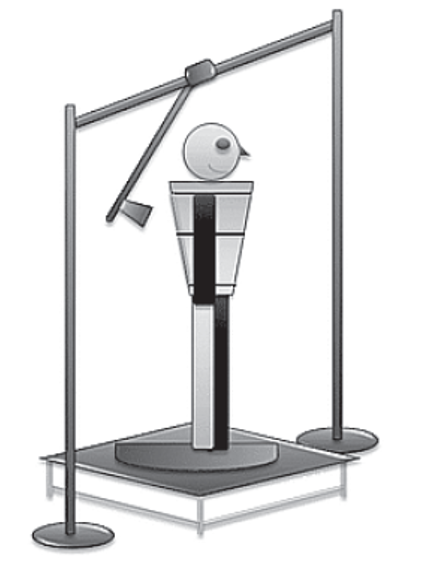
\includegraphics[width=1\linewidth]{images/human.png}
				\caption{Схематическое изображение толкателя
					и положения испытуемого на стабилоплатформе}
			\end{minipage}
			\hfill
			\begin{minipage}[h]{0.66\linewidth}
				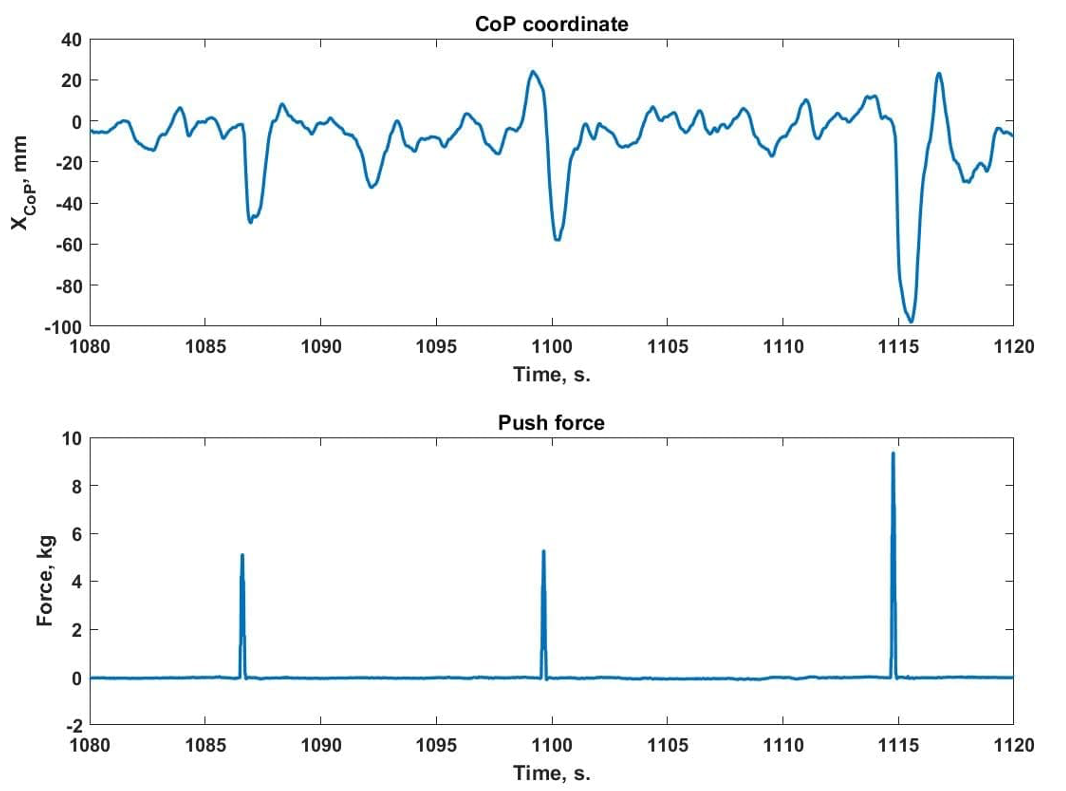
\includegraphics[width=1\linewidth]{images/Pushes.png}
				{\footnotesize
					\caption{Отклонение сагиттальной координаты при различных по силе толчках (данные предоставлены сотрудниками ИМБП РАН) }
				}
			\end{minipage}
		\end{center}
	\end{figure}
\end{frame}

\begin{frame}{Задача быстродействия}
	\begin{columns}
		\column{0.62\textwidth}
		\begin{figure}[h!]
			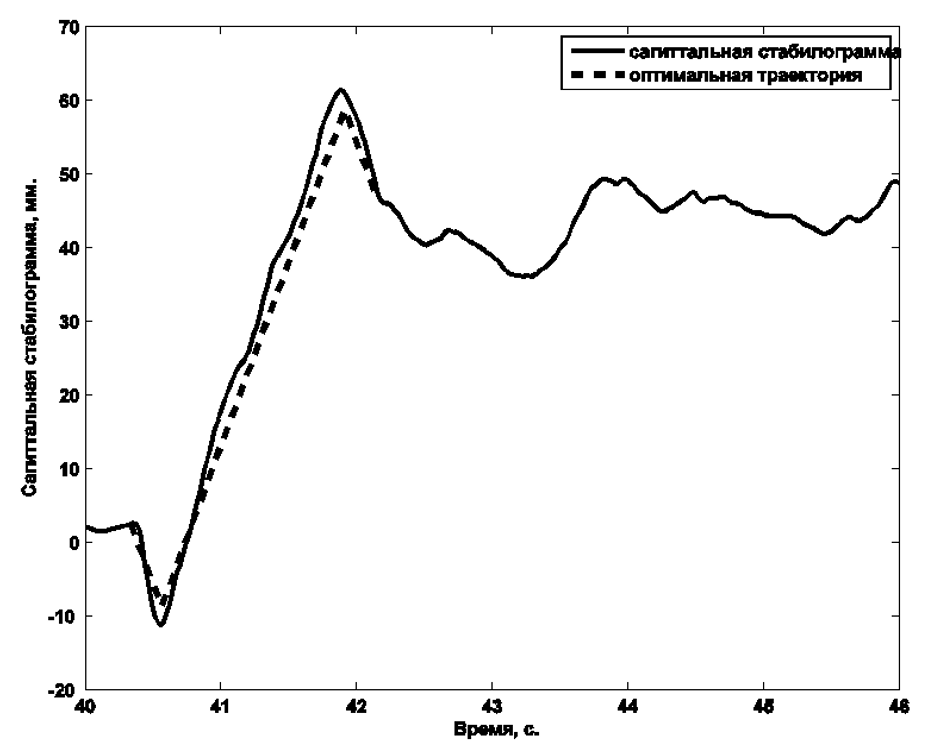
\includegraphics[width=1\linewidth]{images/stabilos.png}
			\caption{Характерный вид сагиттальной стабилограммы при выполнении теста со ступенчатым воздействием}
		\end{figure}
		\column{0.5\textwidth}
		% \column{\dimexpr\paperwidth-2pt}
		В работе рассматривается задача быстродействия для установки
		перевернутого маятника в неустойчивое вертикальное положение
		равновесия. Предполагается сравнение результатов стабилометрических
		проб, при которых человек возвращается в исходную вертикальную
		позу после толчка, с решением этой оптимальной задачи для начальных
		условий, соответствующих моменту времени завершения толчка.
	\end{columns}
\end{frame}

\begin{frame}{Математическая модель}
	\begin{columns}
		\column{0.62\textwidth}
		\begin{figure}[h!]
			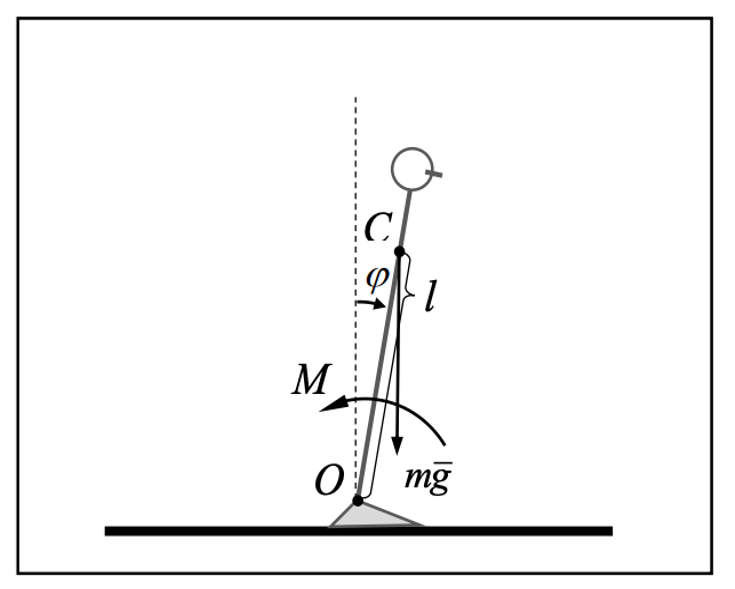
\includegraphics[width=1\linewidth]{images/inverse_pendulum.png}
			\caption{Модель перевернутого маятника}
		\end{figure}
		\column{0.5\textwidth}

		\[
			J\ddot{\varphi}=m_Tgl\varphi+M
		\]
		\[
			\varphi(0)=\varphi_0,\, \dot{\varphi}(0)=\omega_0
		\]
		\[
			\varphi(t)=\varphi_k,\, \dot{\varphi}(t_k)=0
		\]
		\[
			M(0)=M(t_k)=-m_Tgl\varphi_k
		\]
		\[
			U^-\leq\dot{M}\leq U^+
		\]
	\end{columns}
\end{frame}


\begin{frame}{Переход к безразмерным величинам}
	\[
		\theta^{''}=\theta+m;\ m^{'}=u
	\]
	\begin{columns}
		\column{0.3\textwidth}
		\[
			\theta=\frac{\varphi-\varphi_k}{\varphi_\ast},\ \ m=\frac{M-M_f}{m_Tgl\varphi}
		\]
		\column{0.6\textwidth}
		Необходимо решение системы
		перевести из начального положения
		\[
			\theta(0)=1;\ \dot{\theta}(0)=\frac{t_\ast}{\varphi_\ast}\omega_0=\Omega_0;\ m(0)=0
		\]
		в положение
		\[
			\theta(\tau_f)=0;\ \dot{\theta}(\tau_f)=0;\ m(\tau_f)=0
		\]
		с помощью ограниченного управления
		\[
			u^-\le\ u\le\ u^+,\ \text{где } u^-=\frac{U^-}{m_Tgl\varphi_\ast t_\ast}=-u^+
		\]

	\end{columns}
\end{frame}

\begin{frame}{Принцип максимума Понтрягина}
	Система в форме Коши
	\begin{equation}\label{koshisystem}
		\left\{ {\begin{aligned}
					 & \theta^{'} = \omega , \hfill   \\
					 & \omega^{'} = \theta+m , \hfill \\
					 & m^{'} = u . \hfill             \\
				\end{aligned}} \right.
	\end{equation}
	Функция Понтрягина
	\[
		H=\psi_1\cdot\omega+\psi_2\cdot(\theta+m)+\psi_3\cdot u
	\]

	Сопряженная система уравнений
	\begin{equation} \label{7}
		\left\{ {\begin{aligned}
					 & \psi^{'}_1  = - \psi_2\hfill     \\
					 & \psi^{'}_2   = - \psi_1\hfill    \\
					 & \psi^{'}_3   = - \psi_2 . \hfill \\
				\end{aligned}} \right.
	\end{equation}

\end{frame}

\begin{frame}{Анализ сопряженной системы}
	\begin{equation}\label{psisystem}
		\left\{ {\begin{aligned}
					 & \psi_1 = -C_1e^\tau+C_2e^{-\tau}+C_3, \hfill  \\
					 & \psi_2 = C_1e^\tau+C_2e^{-\tau} , \hfill      \\
					 & \psi_3 = -C_1e^\tau+C_2e^{-\tau}+C_3 . \hfill \\
				\end{aligned}} \right.
	\end{equation}
	Анализируя корни уравнения $\psi_3(\tau)=0$, для различной комбинации
	коэффициентов $C_1,C_2,C_3$, получим, что число корней не может быть больше двух. В системе может быть не более двух переключений $u$.
\end{frame}




\begin{frame}{Решение системы на 1 этапе}
	\begin{columns}
		\column{1\textwidth}
		Этап 1. $u=u_*$ начальные условия
		\[
			\theta(0)=1;\ \omega(0)=\Omega_0;\ m(0)=0
		\]
		Решение
		\[
			\left\{ {\begin{aligned}
						 & m_1(\tau) = -\tau  u_*, \hfill                                                               \\
						 & \theta_1(\tau) = \frac{e^\tau+e^{-\tau}}{2}+\frac{\Omega_0-u_*}{2}(e^\tau-e^{-\tau})+\tau u_* , \hfill                            \\
						 & \omega_1(\tau) =\frac{e^\tau-e^{-\tau}}{2}+\frac{\Omega_0-u_*}{2}(e^\tau+e^{-\tau})+u_*   . \hfill                                                                  \\
					\end{aligned}} \right.
		\]
	\end{columns}
\end{frame}
\begin{frame}{Решение системы на 2 этапе}
	\begin{columns}
		\column{1\textwidth}
		Этап 2. $u=u_*$ начальные условия
		\[
			\theta(\tau_1)=\theta_1(\tau_1);\ \omega(\tau_1)=\omega_1(\tau_1);\ m(\tau_1)=m_1(\tau_1)
		\]
		Решение
		\[
			\left\{ {\begin{aligned}
						 & m_2(\tau) = \left(\tau -2 \tau _1\right) u_*, \hfill                                                                                                \\
						 & \theta_2(\tau) = \frac{e^\tau+e^{-\tau}}{2}+\frac{\Omega_0-u_\ast}{2}(e^\tau-e^{-\tau})+u_*(e^{\tau-\tau_1}-e^{-\tau+\tau_1}+2\tau_1-\tau) , \hfill \\
						 & \omega_2(\tau) = \frac{e^\tau-e^{-\tau}}{2}+\frac{\Omega_0-u_\ast}{2}(e^\tau+e^{-\tau})+u_*(e^{\tau-\tau_1}+e^{-\tau+\tau_1}-1) . \hfill            \\
					\end{aligned}} \right.
		\]
	\end{columns}
\end{frame}
\begin{frame}{Решение системы на 3 этапе}
	\begin{columns}
		\column{1\textwidth}
		Этап 3. $u=-u_*$ конечные условия
		\[
			\theta(\tau_f)=0;\ \omega(\tau_f)=0;\ m(\tau_f)=0
		\]
		Решение
		\[
			\left\{ {\begin{aligned}
						 & m_3(\tau) = u_* \left(\tau _f-\tau \right), \hfill                                           \\
						 & \theta_3(\tau) = \frac{1}{2} u_* \left(-e^{\tau -\tau _f}+e^{\tau _f-\tau }-2 \tau _f+2 \tau
						\right), \hfill                                                                                 \\
						 & \omega_3(\tau) =u_*-\frac{u_*}{2}(e^{\tau-\tau_f}+e^{-\tau+\tau_f}) . \hfill                 \\
					\end{aligned}} \right.
		\]
	\end{columns}
\end{frame}

\begin{frame}{Сопряжение уравнений}
	\begin{equation}
		\left\{ {\begin{aligned}
					 & m_2(\tau_2) = m_3(\tau_2), \hfill            \\
					 & \theta_2(\tau_2) =  \theta_3(\tau_2), \hfill \\
					 & \omega_2(\tau_2) = \omega_3(\tau_2) . \hfill \\
				\end{aligned}} \right.
	\end{equation}
	\begin{columns}
		\column{1.2\textwidth}
		{\footnotesize
			\[
				\left\{ {\begin{aligned}
							 & \tau_f=2(\tau_2-\tau_1),                                                                                                                                                                 \\
							 & \frac{e^{\tau_2}+e^{-\tau_2}}{2}+\frac{\Omega_0-u_*}{2}(e^{\tau_2}-e^{-\tau_2})+u_*\left(e^{-\tau_1+\tau_2}-e^{\tau_1-\tau_2}+\frac{e^{\tau_2-\tau_f}-e^{-\tau_2+\tau_f}}{2}\right)=0,   \\
							 & \frac{e^{\tau_2}-e^{-\tau_2}}{2}+\frac{\Omega_0-u_*}{2}(e^{\tau_2}+e^{-\tau_2})+u_*\left(e^{\tau_1-\tau_2}+e^{-\tau_1+\tau_2}+\frac{e^{\tau_2-\tau_f}+e^{-\tau_2+\tau_f}}{2}-2\right)=0. \\
						\end{aligned}} \right.
			\]
		}
	\end{columns}
\end{frame}

\begin{frame}{Замена переменных}
	\[
		x=e^{\tau_1} ,\,\,y=e^{\tau_2} ,\,\,z=e^{\frac{\tau_f}{2}}
	\]
	\begin{equation}\label{fullchanged}
		\left\{ {\begin{aligned}
					 & z=\frac{y}{x}, \hfill                                                                                                              \\
					 & (\Omega_0-u_*)\left( xy-\frac{x}{y}\right)+u_*\left(\frac{x^3}{y}-\frac{y}{x}-\frac{2x^2}{y}+2y\right)+\frac{x}{y}+xy=0, \hfill    \\
					 & (\Omega_0-u_*)\left( xy+\frac{x}{y}\right)+u_*\left(\frac{x^3}{y}+\frac{y}{x}+\frac{2x^2}{y}+2y-4x\right)-\frac{x}{y}+xy=0. \hfill \\
				\end{aligned}} \right.
	\end{equation}
\end{frame}

\begin{frame}{Численные примеры реализации оптимального управления}
	Построим оптимальную траекторию, при следующих значениях параметров

	$m_T=74$кг; $l=0.88$м; $J=\frac{4ml^2}{3}$кг$\cdot$м$^2$
	\[
		t_\ast=\sqrt{\frac{J}{m_Tgl}}=\sqrt{\frac{4l}{3g}}=0.346c
	\]



	Характерное значение для $\varphi_\ast=0.087 \text{ рад}$, для $\omega_0=0.069 \text{ рад/с}$.

	$\Omega_0=\frac{t_\ast}{\varphi_\ast}\omega_0=0.274$

	$u^*_{max}=1.65$

\end{frame}
\begin{frame}{Численные примеры реализации оптимального управления}
	Найдем корни системы \eqref{fullchanged} при $\theta^{'}(0)=\Omega_0$, $\theta^{'}(0)=1.3\Omega_0$ и при $\theta^{'}(0)=0.7\Omega_0$.

	\
	При $\theta^{'}(0)=\Omega_0$: $\tau_1=2.12;\tau_2=4.88;\tau_f=5.51;$

	При $\theta^{'}(0)=1.3\Omega_0$: $\tau_1=2.38,\tau_2=5.41,\tau_f=6.06;$

	При $\theta^{'}(0)=0.7\Omega_0$: $\tau_1=2.06,\tau_2=4.74,\tau_f=5.37.$

\end{frame}

\begin{frame}{Зависимость $m(\tau)$}
	\begin{figure}[h!]
		\centering
		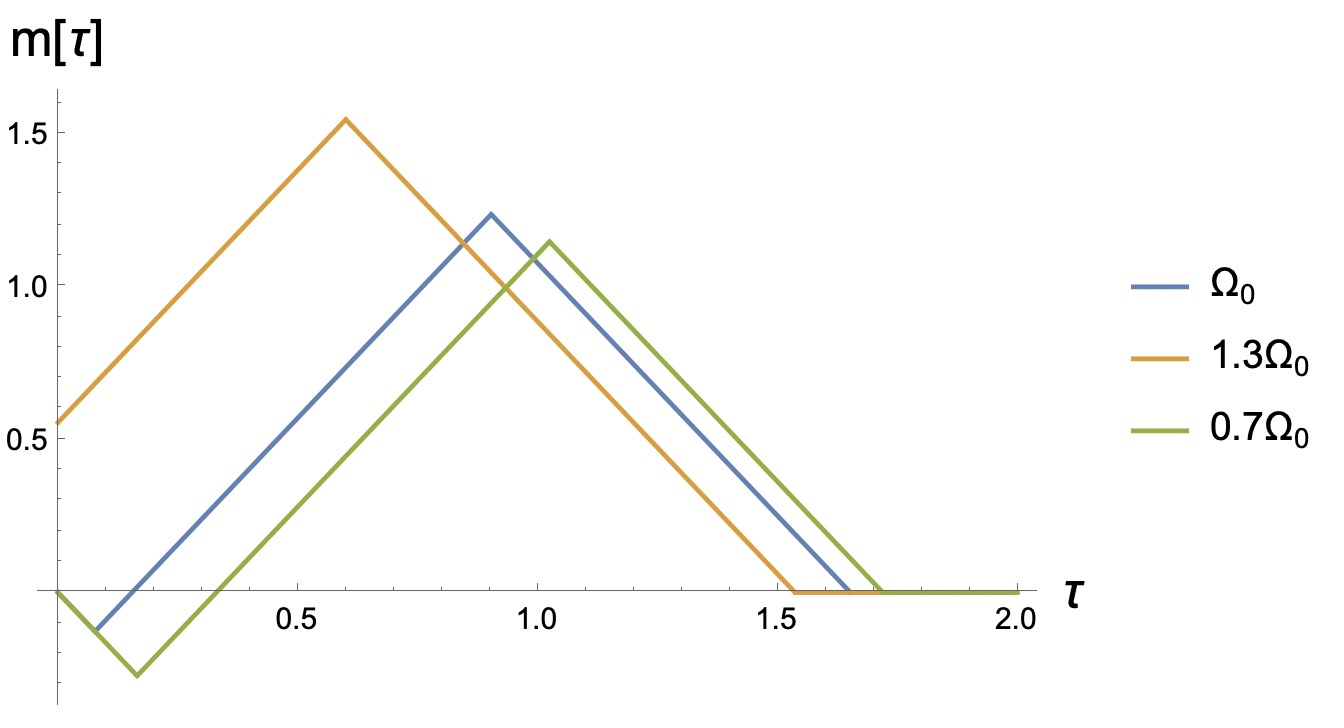
\includegraphics[width=1.0\linewidth]{images/m.jpeg}
		\caption{Зависимость $m(\tau)$}
		\label{fig:m}
	\end{figure}
\end{frame}
\begin{frame}{Зависимость $\Theta(\tau)$}
	\begin{figure}[h!]
		\centering
		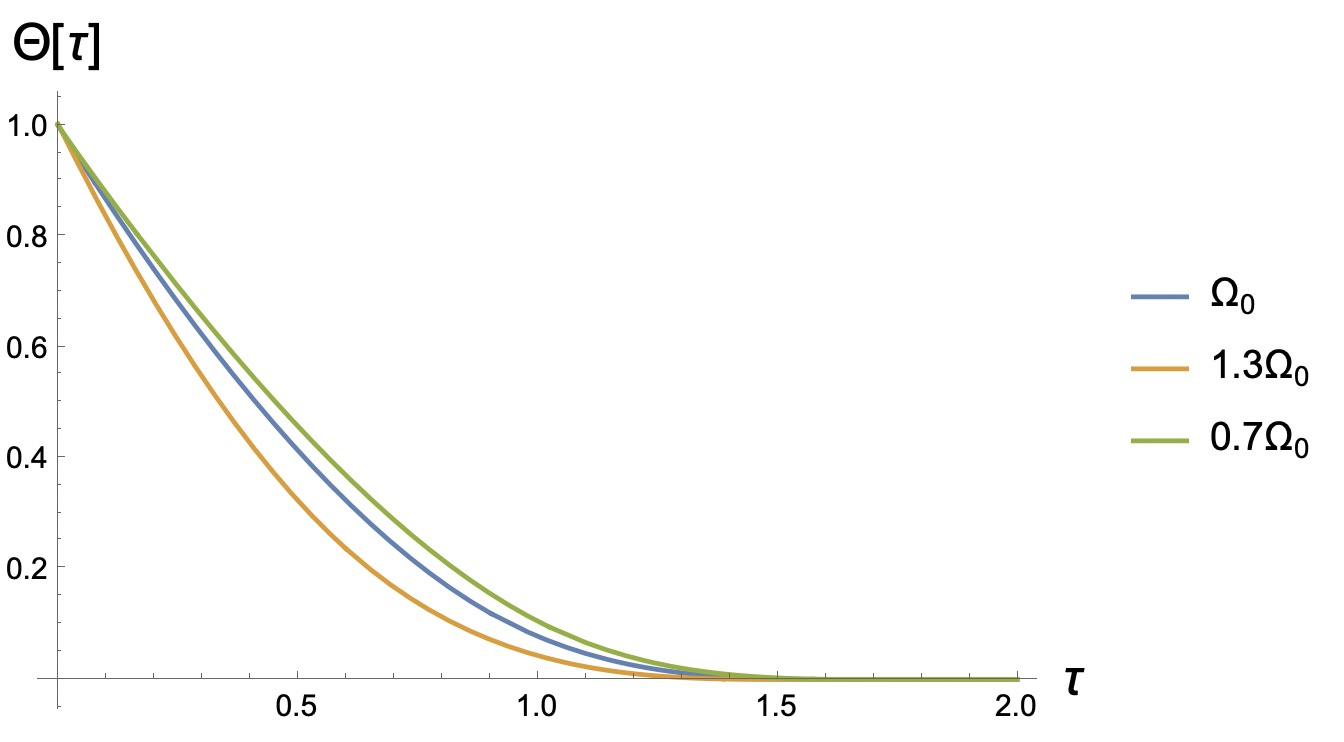
\includegraphics[width=1.0\linewidth]{images/theta.jpeg}
		\caption{Зависимость $\Theta(\tau)$}
		\label{fig:theta}
	\end{figure}
\end{frame}
\begin{frame}{Зависимость $\omega(\tau)$}
	\begin{figure}[h!]
		\centering
		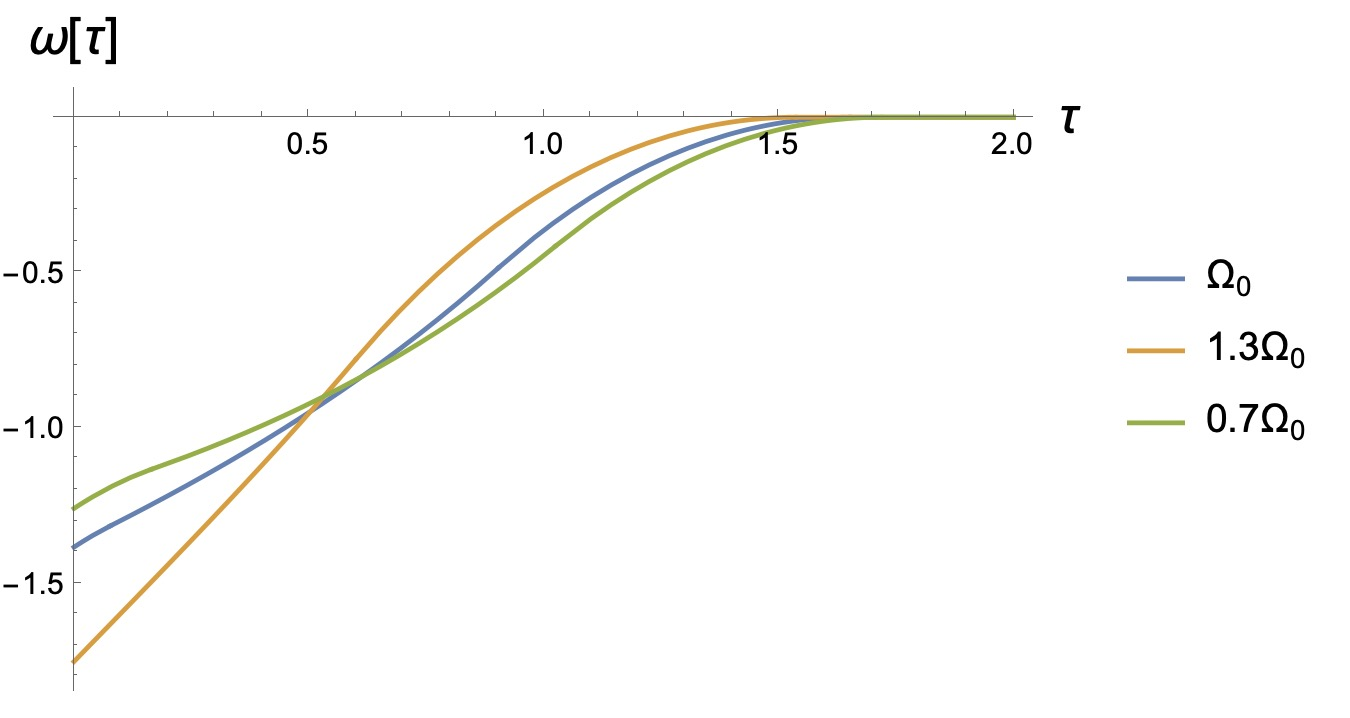
\includegraphics[width=1.0\linewidth]{images/omega.jpeg}
		\caption{Зависимость $\omega(\tau)$}
		\label{fig:omega}
	\end{figure}
\end{frame}

\begin{frame}{Заключение}
	В курсовой работе были представлены оптимальные алгоритмы управления
	движением позой человека при толчке, основанные на модели
	«перевернутого маятника». Построенные алгоритмы решали задачу наискорейшего возвращения человека в исходную вертикальную позицию.
	В задаче ставилось ограничение на скорость изменения момента в голеностопном суставе.
	\begin{itemize}
		\item Показано, что решение оптимальной задачи быстродействия при ограниченной скорости изменения момента в голеностопном суставе может иметь решение, которое качественно совпадает с картиной, наблюдаемой в стабилометрических исследованиях.
		\item Время необходимое для восстановления исходной позы получилось соизмеримым с реальным времени возвращения после толчка.
	\end{itemize}

\end{frame}

\end{document}